%
% Шаблон для ВКР бакалавра 2023
%

\documentclass[a4paper,12pt]{article}
\usepackage{vkriate}

% Настройки для окружений с подчеркиваниями для подписей и пр.
\setFRMfontencoding{T2A}
\setFRMdfontencoding{T2A}
% thanks to A.Starikov
\setFRMfontfamily{cmr}
\setFRMdfontfamily{ptm}
\setFRMdfontsize{10pt}

% задает длину поля для подписи на титульной странице
\newFRMfield{xtitlesign}{32mm}

% поле для факультета или кафедры
\newFRMfield{fcath}{65mm}

%имя файла с библиографией в формате BibTex
\addbibresource{rbiblio.bib}

\begin{document}

% счетчики страниц, рисунков, таблиц
\regtotcounter{page}
\regtotcounter{figure}
\regtotcounter{table}

\renewcommand{\refname}{\centerline{СПИСОК ИСПОЛЬЗОВАННЫХ ИСТОЧНИКОВ}} 
\renewcommand{\contentsname}{\centerline{СОДЕРЖАНИЕ}} 
%\renewcommand{\refname}{Список источников}  % По умолчанию "Список литературы" (article)
%\renewcommand{\bibname}{Литература}  % По умолчанию "Литература" (book и report)

% титульная страница
\thispagestyle{empty}
\begin{center} \small
\textbf{МИНИСТЕРСТВО НАУКИ И ВЫСШЕГО ОБРАЗОВАНИЯ\\ РОССИЙСКОЙ ФЕДЕРАЦИИ}\\
ФЕДЕРАЛЬНОЕ ГОСУДАРСТВЕННОЕ АВТОНОМНОЕ ОБРАЗОВАТЕЛЬНОЕ УЧРЕЖДЕНИЕ
ВЫСШЕГО  ОБРАЗОВАНИЯ\\
«Национальный исследовательский ядерный университет «МИФИ»\\
\textbf{Обнинский институт атомной энергетики} – \\
филиал федерального государственного автономного образовательного учреждения высшего\\
образования «Национальный исследовательский ядерный университет «МИФИ»\\
(ИАТЭ НИЯУ МИФИ)
\end{center}
%\vfill
\medskip

% Направление подготовки следует уточнять,
% магистры и бакалавры могут иметь разные наименования
\begin{center}
\begin{tabular}{rl}
Отделение & \useFRMfield{fcath}[\large Интеллектуальные кибернетические системы] \\ 
%Направление подготовки & \useFRMfield{fcath}[\large Информационные системы и технологии] \\ 
\end{tabular} 
\end{center}

\vfill

\large 

\begin{center}
\textbf{\Large Выпускная квалификационная работа --- } \\
\textbf{\Large бакалаврская работа}\\
	
	\medskip

{ \normalsize
по направлению подготовки  \textbf{09.03.02 Информационные  системы и технологии}\\

Направленность (профиль) \textbf{Информационные технологии}
}	
\vfill
\vfill
\medskip

\textbf{\Large 
		<<Разработка ИС автоматизированного статистического анализа данных, полученных при КГО стендовым методом на реакторах типа ВВЭР>>
	}
	
\end{center}

\vspace{1cm}

\begin{center}
\begin{tabular*}{\textwidth}{p{78mm}p{33mm}p{64mm}}
	Выполнил:\\студент гр. ИС2-Б20 & \useFRMfield{xtitlesign} & Костевич А.Е.\\
	& & \\
% должность, научная степень руководителя
	Руководитель ВКР,\\старший преподаватель ОИКС & \useFRMfield{xtitlesign} & Радаев А.В. \\
	& & \\
	
	Нормоконтроль\\ доцент отделения ИКС, к.ф.-м.н. & \useFRMfield{xtitlesign} &  Качанов~Б.В. \\
	& & \\
	% Если нужно добавить консультанта - раскомментируйте две строчки ниже
	%Консультант ВКР бакалавра\\организация, должность, звание  & \useFRMfield{xtitlesign} & К.О.Нсультант\\
	%& & \\
%	Рецензент\\к.ф.-м.н.,   & \useFRMfield{xtitlesign} & В.А. Чепурко\\
	
	& & \\
	Выпускная квалификационная \\ работа допущена к защите & \useFRMfield{xtitlesign} &  \\
	& & \\
	Руководитель\\ образовательной программы \\
	09.03.02 Информационные системы и технологии\\
	канд. тех. наук  & \useFRMfield{xtitlesign} &Мирзеабасов~О.А. \\
	
\end{tabular*}
\end{center}

\vfill
\large

\begin{center}
Обнинск, 2024 г
\end{center}

\onehalfspacing

\pagebreak

% реферат
\thispagestyle{empty}

\section*{\centering РЕФЕРАТ}

\thispagestyle{empty} % страница реферата не нумеруется

Работа \total{page} стр., \total{table} табл., \total{figure} рис., \totalmycitecounts ист. 

РАЗРАБОТКА ИНФОРМАЦИОННОЙ СИСТЕМЫ
АВТОМАТИЗИРОВАННОГО СТАТИСТИЧЕСКОГО АНАЛИЗА ДАННЫХ,
ПОЛУЧЕННЫХ ПРИ ПРОВЕДЕНИИ КГО СТЕНДОВЫМ МЕТОДОМ ДЛЯ
РЕАКТОРОВ ТИПА ВВЭР.

Текст реферата должен отражать:
\begin{itemize}
\item объект исследования;
\item предмет исследования;
\item цель работы;
\item метод или методологию проведения работы;
\item научную новизну исследования (для магистерских диссертаций);
\item практическую значимость результатов работы;
\item степень внедрения (при наличии справки о внедрении);
\item экономическую эффективность работы.
\end{itemize}
Текст реферата должен размещаться на одном листе (странице).

\pagebreak
\thispagestyle{empty}

\section*{\centering ОПРЕДЕЛЕНИЯ}

\thispagestyle{empty} % страница определений не нумеруется

Реперный радионуклид --- радионуклид, по выходу которого из твэла в
теплоноситель первого контура судят о герметичности оболочки твэла, так как
он обладает ядерно-физическими и химическими характеристиками,
позволяющими надежно регистрировать его в условиях эксперимента.

Негерметичный твэл - твэл, в оболочке которого имеется повреждение,
приводящее к выходу продуктов деления из него.

Негерметичная ТВС --- ТВС, в составе которой имеются негерметичные твэлы.

\pagebreak

\section*{\centering ОБОЗНАЧЕНИЯ И СОКРАЩЕНИЯ}

\thispagestyle{empty} % страница обозначений и сокращений не нумеруется

БВ --- Бассейн выдержки.

ВВЭР --- Водо-водяной энергетический реактор.

КГО --- Контроль герметичности оболочек.

ПД --- Продукты деления.

СОДС --- Система обнаружения дефектных сборок.

ТВС --- Тепловыделяющая сборка.

\pagebreak

% титульная страница - номер 1, остальные страницы до Содержания не нумеруются
\tocloftpagestyle{empty}

\tableofcontents
% если нужно добавить "Стр." над номерами страниц - раскомментируйте следующую команду
%\addtocontents{toc}{~\hfill\textbf{Стр.}\par}

\thispagestyle{empty}

\pagebreak

\setcounter{page}{3}

\section*{\centering ВВЕДЕНИЕ}
\addcontentsline{toc}{section}{ВВЕДЕНИЕ}
% пример введения

Атомные электростанции играют ключевую роль в современной
энергетике. Однако сопутствующие ядерной энергетике риски требуют
непрерывного совершенствования методов контроля и обслуживания ядерных установок.

В частности, одним из значимых аспектов эксплуатации ядерных реакторов является контроль герметичности оболочек тепловыделяющих
элементов. В настоящее время анализ данных, полученных при проведении
КГО, частично осуществляется в ручном режиме, что требует значительных ресурсов времени и труда. Более того, этот подход подвержен человеческим ошибкам и может ограничивать возможности в проведении анализа данных с высокой точностью и скоростью.

Как известно, одним из недостатков реактора типа ВВЭР является
невозможность перегрузки топлива без остановки реактора и ошибка,
допущенная при принятии решения относительно герметичности ТВС, может повлечь за собой существенные экономические издержки.

Цель настоящей работы заключается в разработке программного обеспечения, работа которого направлена на повышение эффективности
и достоверности результатов КГО, а также снижение трудовых затрат.

В данной работе будет проведен обзор существующего метода обработки результатов КГО, приведены предложения по его автоматизации, а также описан процесс создания прототипа программного обеспечения.
%\cite{SoetaertRJ2010}.
%\cite{kotelnikov}  % текст введения в файле intro.tex
\pagebreak

%\input{Post_zad}
\pagebreak
% первая часть

\section{Обзор существующей методики проведения процедуры КГО стендовым методом}

\subsection{Основные положения}

В данной работе рассматривается метод КГО в пеналах СОДС~\cite{RD}, который является одним из наиболее надёжных способов определения негерметичных ТВС. СОДС входит в состав обязательного оборудования всех действующих и проектируемых АЭС с реактором ВВЭР.

Метод основан на измерении утечки ПД из-под оболочек твэлов путем гамма-спектрометрического анализа изотопного состава проб воды, отбираемой из контура циркуляции СОДС, по активностям реперных радионуклидов $^{131}$I, $^{134}$Cs, $^{136}$Cs, $^{137}$Cs и $^{133}$Xe. Инициирование выхода радионуклидов в воду стенда КГО осуществляется посредством изменения давления в процессе выдержки ТВС в этой воде --- настаивании.

\subsection{Процедура проведения КГО стендовым методом}
1. Процедура проведения КГО начинается проведения испытаний для каждой ТВС в пеналах СОДС с последующим отбором проб воды. 

Проверка ТВС проводится при циркуляции воды по контуру стенда КГО без ее замены и состоит из двух циклов:
\begin{itemize}
\item Настаивание ТВС при изыбыточном (верхнем) давлении в контуре от 4,5 * 10$^{5}$ Па до 6,0 * 10$^{5}$ Па продолжительностью 5 минут.

\item Настаивание ТВС при избыточном (нижнем) давлении в контуре от 1,0 * 10$^{5}$ Па до 1,5 * 10$^{5}$ Па до полного перемешивания (не менее 15 минут).
\end{itemize}

С целью соблюдения одинаковых условий испытаний требуется, чтобы значения верхнего и нижнего избыточного давления были одинаковыми при проверке всех ТВС. 

2. После завершения настаивания ТВС производится отбор пробы воды из контура стенда КГО.

3. В каждой $j$-ой пробе воды, взятой из стенда КГО при испытании $j$-ой ТВС, на спектрометрической установке измеряются значения удельной активности и приводятся на момент останова реактора:
\begin{itemize}
\item $A_{j,кго}^{i}$ --- реперных $i$-х радионуклидов продуктов деления ($^{131}$I, $^{134}$Cs, $^{136}$Cs, $^{137}$Cs и $^{133}$Xe)

\item $A_{j,кго}^{i'}$ --- радионуклида продуктов коррозии(ПК) ($^{54}$Mn или $^{58}$Co, $^{60}$Co, $^{51}$Cr, $^{59}$Fe).
\end{itemize}

4. Для учета фоновой активности радионуклидов йода, цезия и
продуктов коррозии периодически производится измерение их активности
в воде, подаваемой в стенд КГО (с каждой вновь приготовленной порцией
раствора борной кислоты на СВО), и в бассейне выдержки (один раз в
сутки).

5. Проверка фоновой составляющей за счет загрязнения стенда
радиоактивными продуктами (холостая проба) производится перед началом
работ по КГО, а также периодически (не реже одного раза в сутки). Для этого
без загрузки ТВС в пенал проводятся все операции по промывке контура и
настаиванию с отбором и анализом пробы.

6. Итогом проведения спектрометрического анализа проб воды является
таблица значений, в которых для каждой $j$-ой ТВС приводятся в соответствие
значения активности $A_{j,кго}^{i}$ каждого из регистрируемых реперных радионуклидов
и $A_{j,кго}^{i'}$ продуктов коррозии. Статистический анализ результатов
измерения проводится для ТВС, в пробах которых значимо регистрировались
ПД. Результаты измерений ТВС, при проверке которых реперные ПД не
регистрировались, из статистического расчета исключаются.

\subsection{Обработка результатов}
1. Анализ герметичности ТВС, согласно~\cite{RD}, основан на выборочном поиске выбросов методом "трёх сигм".

2. Основными реперными радионуклидами, по которым устанавливается наличие(отсутствие) негерметичных твэлов в ТВС являются $^{131}$I, $^{134}$Cs, $^{137}$Cs. Наличие в контролируемой пробе $^{136}$Cs и(или) $^{133}$Xe, значимо превышающих их содержание в холостых пробах, является однозначным основанием для включение ТВС в список подозрительных, требующих как минимум дополнительной проверки.

3. Полученные значения представляются в графическом виде в такой
хронологической последовательности, в какой ТВС проверялись в стенде
КГО. Примеры графического представления результатов КГО приведены на
рисунках~\ref{fig:ris1} и~\ref{fig:ris2}. На основании визуального анализа этих данных на графике
может быть сделано заключение, относятся ли они к одному статистическому
распределению. Таким способом проводится оценка соблюдения одинаковых
условий проверки всех ТВС.\label{distribution} Если условия менялись с течением времени (на
практике так происходит почти всегда), то производится разделение исходных данных на выборки, которые относятся к одному статистическому распределению.

\begin{figure}[H]
	\centering
	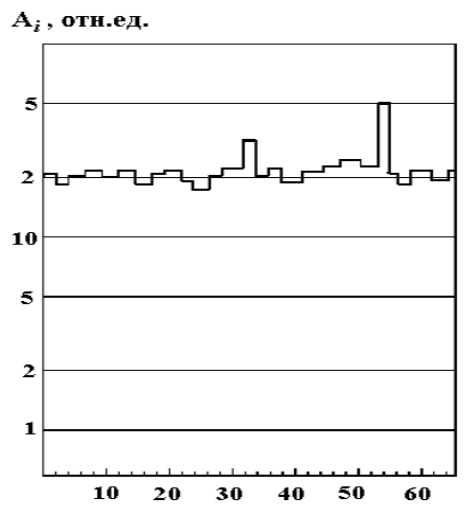
\includegraphics[width=0.5\linewidth]{pics/ris1} % изображения хранятся в подкаталоге pics
	\caption{Графическое хронологическое представление данных, принадлежащих к одному распределению.~\cite{RD}}
	\label{fig:ris1} % эта метка позволяет ссылаться на рисунок в тексте
\end{figure}

\begin{figure}[H]
	\centering
	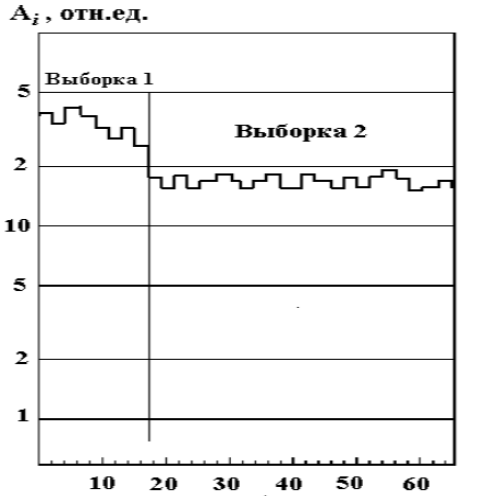
\includegraphics[width=0.5\linewidth]{pics/ris2} % изображения хранятся в подкаталоге pics
	\caption{Графическое хронологическое представление данных, принадлежащих к различным распределениям.~\cite{RD}}
	\label{fig:ris2} % эта метка позволяет ссылаться на рисунок в тексте
\end{figure}

4. Для каждой полученной совокупности данных, относящихся к одному
и тому же статистическому распределению, вычисляются $\overline{A}_{кго}^{i}$ --- среднеарифметические значения удельной активности радионуклидов $^{131}$I (и $^{134}$Cs, $^{136}$Cs, $^{137}$Cs, $^{133}$Xe) и $\overline{A}_{кго}^{i'}$ --- среднеарифметическое значение удельной активности $^{54}$Mn (или $^{58}$Co, $^{60}$Co, $^{51}$Cr, $^{59}$Fe), по формулам~\ref{eq:Mean} и~\ref{eq:corosionMean}:

\begin{equation} \label{eq:Mean}
	\overline{A}_{кго}^{i} = \frac{1}{N}\sum_{j=1}^{N}A_{j,кго}^{i}.
\end{equation}

\begin{equation} \label{eq:corosionMean}
	\overline{A}_{кго}^{i'} = \frac{1}{N}\sum_{j=1}^{N}A_{j,кго}^{i'}.
\end{equation}

Кроме того, рассчитывают соответствующие им среднеквадратичные
отклонения (стандартные статистические неопределенности) по формулам~\ref{eq:Std} и~\ref{eq:corosionStd}:

\begin{equation} \label{eq:Std}
	\sigma_{{A}_{кго}^{i}} = \sqrt{\frac{1}{N-1}\sum_{j=1}^{N}(A_{j,кго}^{i} - \overline{A}_{кго}^{i})^2},
\end{equation}
	
\begin{equation} \label{eq:corosionStd}
	\sigma_{{A}_{кго}^{i'}} = \sqrt{\frac{1}{N-1}\sum_{j=1}^{N}(A_{j,кго}^{i'} - \overline{A}_{кго}^{i'})^2},
\end{equation}

где N --- количество проверенных ТВС.

5. Если N > 10, то ТВС, для которых выполняется условие~\ref{eq:3sigma} являются герметичными.

\begin{equation} \label{eq:3sigma}
	A_{j,кго}^{i} \leq \overline{A}_{кго}^{i} + 3*\sigma_{{A}_{кго}^{i}}.
\end{equation}

ТВС, для которых одновременно выполняются условия~\ref{eq:3sigma_non_hermetic} и~\ref{eq:3sigma_corosion} являются негерметичными.

\begin{equation} \label{eq:3sigma_non_hermetic}
	A_{j,кго}^{i} > \overline{A}_{кго}^{i} + 3*\sigma_{{A}_{кго}^{i}}.
\end{equation}

\begin{equation} \label{eq:3sigma_corosion}
	A_{j,кго}^{i'} \leq \overline{A}_{кго}^{i'} + 3*\sigma_{{A}_{кго}^{i'}}.
\end{equation}

Важно отметить, что активности радионуклидов ПК измеряются с целью учёта при анализе данных. ПК, образующиеся в конструкционных материалах реактора по мере эксплуатации, переносятся по теплоносителю и могут откладываться на ТВС, что влечёт за собой повышение активности в том числе и реперных ПД~\cite{corosion}. Именно поэтому повышение активности реперных ПД совместно с активностями ПК может являться признаком некачественной отмывки ТВС при подготовке к проведению испытаний.

6. Если количество ТВС в выборке N < 10, то в формулах~\ref{eq:3sigma}-\ref{eq:3sigma_corosion}  в качестве коэффициента при $\sigma$  вместо значения 3 используются коэффициенты Стьюдента, приведенные в таблице~\ref{tab:Student}, для доверительной вероятности 0,95.
\begin{table}[H]
	\caption{Значения коэффициента Стьюдента в зависимости от количества проверенных ТВС и вероятности, с которой ТВС могут быть отнесены к разряду имеющих негерметичные твэлы} \label{tab:Student}
	\centering
	\begin{tabular}{|c|c|c|c|}
		\hline Кол-во ТВС & 0,95 & 0,99 & 0,999 \\ 
		\hline  2 & 12,7 & 66,7  & 637 \\ 
		\hline 3 &  4,30 &  9,93 & 31,6 \\ 
		\hline 4 &  3,18 &  5,84 & 12,9 \\ 
		\hline 5 &  2,78 &  4,60 & 8,61 \\ 
		\hline 6 &  2,57 &  4,03 & 6,86 \\ 
		\hline 7 &  2,45 &  3,71 & 5,96 \\ 
		\hline 8 &  2,36 &  3,50 & 5,41 \\ 
		\hline 9 &  2,31 &  3,36 & 5,04 \\ 
		\hline 10 & 2,26 &  3,25 & 4,78 \\ 
		\hline 
	\end{tabular} 
\end{table} 

7. Заключение о герметичности ТВС, для которых при выполнении
условия \ref{eq:3sigma_corosion} условие \ref{eq:3sigma_non_hermetic} выполняется не для всех основных реперных ПД($^{131}$I, $^{134}$Cs, $^{137}$Cs), производится с учетом дополнительной информации: наличие
(величина удельной активности) в пробах КГО других реперных ПД($^{136}$Cs, $^{133}$Xe), а также соотношения активности $^{134}$Cs и $^{137}$Cs с учётом выгорания.

8. Если в результате вычислений выявлены ТВС, содержащие твэлы с
негерметичными оболочками, то проводится повторный расчет величин по формулам~\ref{eq:Mean}-\ref{eq:corosionStd} и проверка по условиям~\ref{eq:3sigma_non_hermetic} и~\ref{eq:3sigma_corosion} для остальных ТВС.

9. Повторение расчетов и проверок производится до тех пор, пока все ТВС, включаемые в повторную проверку, не будут удовлетворять условию~\ref{eq:3sigma}.\label{povtor}

10. После завершения последовательно проведенных расчетов и проверок
повторный КГО твэлов проводится для следующих ТВС:
\begin{itemize}
	\item для которых выполняется условие \ref{eq:3sigma_non_hermetic} для основных реперных ПД и одновременно не выполняется условие \ref{eq:3sigma_corosion};
	\item для которых выполняется условие \ref{eq:3sigma_non_hermetic}, но проверенных сразу после ТВС, для которых также выполняется условие \ref{eq:3sigma_non_hermetic}.
	\item для которых выполняются условие \ref{eq:3sigma_non_hermetic} и условие \ref{eq:3sigma_corosion}, но удельная активность $^{134}$Cs и $^{137}$Cs в пробе не превышала 7,4*10$^{4}$ Бк/кг
	(2*10$^{-6}$ Ки/кг).
\end{itemize}

11. Результат повторной проверки включается в анализируемую совокупность вместо первичного, если он качественно отличается от него. 

\subsection{Учет выгорания топлива ТВС}

Радионуклид $^{137}$Cs (t$_{1/2}$=30 лет) является конечным продуктом
радиоактивного бета-распада предшественников в цепочке радиоактивного
распада. Влияние других мод образования $^{137}$Cs несущественно, так что
количество атомов этого радионуклида в топливе и под оболочкой твэла
оказывается прямо пропорционально выгоранию.

Радионуклид $^{134}Cs$ (t$_{1/2}$=2,06 лет) образуется преимущественно за счет реакции (n,$\gamma$) на ядрах стабильного изотопа $^{133}Cs$, который является последним членом цепочки радиоактивного распада и накапливается в топливе практически линейно с выгоранием.

Поскольку образование $^{134}Cs$ из $^{133}Cs$ в первом приближении линейно с выгоранием, общее количество 134Cs оказывается близким к квадратичной функции от выгорания, естественно, с учетом радиоактивного распада. Таким образом, соотношение активностей $^{134}Cs$ и $^{137}Cs$ в топливе и под оболочкой оказывается значимо зависящим от выгорания.
При проведении КГО на остановленном реакторе в пеналах СОДС
определение соотношения удельных активностей радионуклидов $^{134}Cs$ и $^{137}Cs$ в пробах КГО может быть использовано в качестве индикатора для дополнительной проверки факта обнаружения ТВС с негерметичными твэлами.

1. Для ТВС, в которых при выполнении условия (7) условие (6)
выполняется не для всех контролируемых реперных ПД, строится
коэффициент, равный отношению отношению удельных активностей $^{134}Cs$ и
$^{137}Cs$ в j-ой пробе стенда КГО:
\begin{equation} \label{eq:Kcs}
	{K}_{кго}^{j} = \frac{A_{j,кго}^{^{134}Cs}}{A_{j,кго}^{^{137}Cs}}.
\end{equation}

На основе сопоставления определенных по формуле (8)
коэффициентов ${K}_{кго}^{j}$ - соотношений измеренных удельных активностей $^{134}$Cs и $^{137}$Cs в пробах от ТВС, определенных как негерметичные, с кривой, приведенной на рисунке~\ref{fig:ris3} определяются расчетные выгорания топлива ТВС с негерметичными твэлами.

\begin{figure}[H]
	\centering
	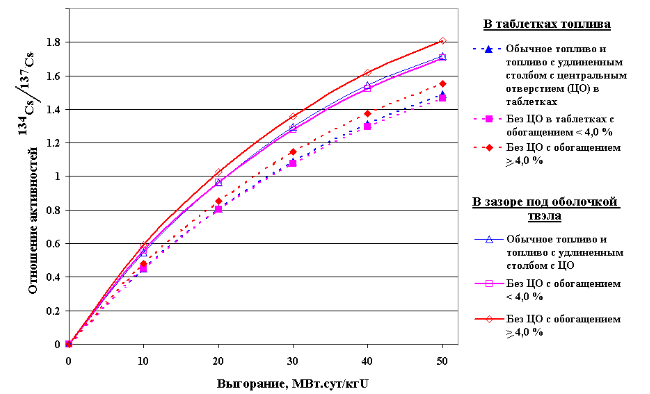
\includegraphics[width=1\linewidth]{pics/ris3} % изображения хранятся в подкаталоге pics
	\caption{Расчетные соотношения активностей радионуклидов $^{134}$Cs и $^{137}$Cs в топливе и в зазоре под оболочкой твэлов в функции выгорания для типичных историй облучения топлива реакторов ВВЭР-1000.~\cite{RD}}
	\label{fig:ris3} % эта метка позволяет ссылаться на рисунок в тексте
\end{figure}

2. Совпадение (с учетом неопределенностей) полученных таким образом
выгораний топлива с выгораниями топлива этих же ТВС по данным
физических расчетов (с учетом неравномерности энерговыделения и
выгорания по высоте и радиусу кассеты) является дополнительным фактом,
подтверждающим наличие негерметичных твэлов в составе контролируемых
ТВС.  % первая глава - в файле part1.tex
\pagebreak
% вторая часть
\section{Предложения по улучшению методики обработки данных}

\subsection{Проблемы существующего подхода}
Рассмотрев методику проведения процедуры КГО согласно\cite{RD} можно выделить несколько замечаний, которые можно пересмотреть:

1. Метод анализа данных, приведённый в параграфе 1.3, основывается на поиске выбросов по правилу "3 сигм". Данное правило утверждает, что  абсолютная величина отклонения нормально распределённой случайной величины от её математического ожидания не превосходит трёх среднеквадратичных отклонений с вероятностью\cite{KremerMatstat}:
\begin{equation} \label{eq:3sigma_rule}
	P(|X - m| < 3\sigma)  = 0,9973
\end{equation}

Проблема этого метода заключается в том, что он применим для выборок, значения которых извлечены из нормально распределённых генеральных совокупностей. Но в случае проведения КГО(согласно разделу 1) нет достаточных оснований утверждать, что все значения активностей будут распределены по нормальному закону. Следовательно, требуется проверить характер распределения для каждой выборки с целью установления корректности применения метода "3 сигм".

Кроме того, среднее и среднеквадратическое отклонение, рассчитываемые в данном методе, также изменяются под воздействием аномальных значений, что приводит к маскировке выбросов\cite{emissions}. Следовательно, имеет смысл рассмотреть альтернативы, например метод межквартильного размаха(IQR).

2. Процедура КГО с учётом времени и объёма испытаний может проходить до нескольких недель. С течением времени в БВ, а также в воде, подаваемой на стенд КГО, может изменяться концентрация борной кислоты с целью борного регулирования, что негативно сказывается на однородности условий проведения испытаний. В связи с этим значения активностей ПД, полученные в разное время, могут принадлежать разным статистическим распределениям, следовательно, анализироваться должны отдельно. 

Согласно пункту 1.3.3, разделение на выборки происходит "На основании визуального анализа"\ графических данных. Хочу отметить, что в изучаемой методике существует способ анализа полученных выборок на принадлежность к одному статистическому распределению с целью объединения нескольких выборок, но он не учитывает анализ на корректность разбиения исходных данных. В связи с вышеперечисленным возникает необходимость проверки данных в выборках, полученных на основании визуального анализа.

3. Описанный процесс анализа данных производится в ручном режиме с использованием программного комплекса Excel. Автоматизация этого процесса позволит снизить вероятность ошибок, ведущих к преждевременной остановке реактора, а также снизить потребность во временных и трудовых затратах.

\subsection{Предложения по улучшению}

\subsubsection{Метод IQR}

Учитывая изложенное в 2.1.1, в качестве альтернативы методу "3 сигм"\ имеет смысл рассмотреть метод поиска выбросов с помощью межквартильного размаха(Interquartile range/IQR).

Межквартильный размах (IQR) — это статистическая мера, равная разности между первым и третьим квартилями распределения (25-м и 75-м процентилями). Первый квартиль (Q1) — это значение, ниже которого находится 25\% данных, а третий квартиль (Q3) — это значение, ниже которого находится 75\% данных. Можно так же сказать, что интерквартильный размах это половина выборки, центрированная относительно медианы. 

Этот показатель полезен для оценки изменчивости признака в асимметричных распределениях или наборах данных с выбросами. Интерквартильный размах является устойчивым(робастным) аналогом дисперсии, поскольку не подвержен влиянию аномальных значений. Именно поэтому он является наиболее перспективным аналогом методу "3 сигм". 
Таким образом, интерквартильный размах позволяет обнаруживать аномальные значения, являясь альтернативой среднеквадратическому отклонению, которое эффективно только для нормально распределенных данных. IQR — это непараметрическая оценка, что делает его применимым для анализа данных любого распределения.

В современных практиках поиска выбросов с использованием межквартильного размаха применяется следующий метод расчёта критических значений:
\begin{equation} \label{eq:IQRmin}
	X^{min}  = Q1-1.5*IQR
\end{equation}

\begin{equation} \label{eq:IQRmax}
	X^{max}  = Q3+1.5*IQR
\end{equation}


На рисунке~\ref{fig:ris6} приведена иллюстрация коэффициента IQR для нормального распределения.

\begin{figure}[H]
	\centering
	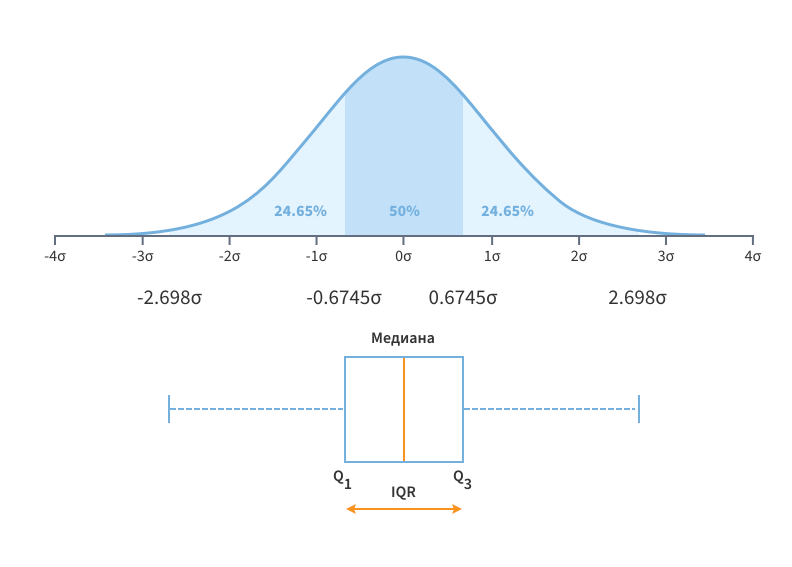
\includegraphics[width=1\linewidth]{pics/ris6} % изображения хранятся в подкаталоге pics
	\caption{Графическое представление межквартильного размаха на примере нормального распределения.}
	\label{fig:ris6} % эта метка позволяет ссылаться на рисунок в тексте
\end{figure}

Из рисунка~\ref{fig:ris6} видно, что данный подход в случае нормального распределения охватывает интервал:
\begin{equation} \label{eq:IQRP}
	P(|X^{min/max} - X| < 2.698\sigma)  = 0,9545
\end{equation}

%Использование этого метода в качестве альтернативы методу "3 сигм"\ с точностью, требуемой в условии \ref{eq:3sigma_rule}, требует замену коэффициента при IQR в формулах~\ref{eq:IQRmin}-\ref{eq:IQRmax}.

%\begin{equation} \label{eq:IQR}
%	P(Q3+1.7*IQR - X < 3\sigma)  = 0,9973
%\end{equation}

\subsubsection{U-критерий Манна-Уитни}

\subsubsection{Критерий Шапиро-Уилка}

\subsubsection{Критерий Стьюдента для независимых выборок}


% 3. Исходя из изложенного в 1.3.1-1.3.2 требуется разделять исходные данные на выборки, принадлежащие как минимум одному статистическому распределению, в идеальном случае требуется, чтобы выборка подчинялась нормальному закону распределения. % вторая глава - в файле part2.tex
\pagebreak

% если есть еще разделы - сохраните их в соответствующих файлах и раскомментируйте строки ниже, при необходимости добавьте еще
%% вторая часть

\section{Проектирование приложения с учётом внесённых предложений}

\subsection{Требования к проектируемому приложению}\label{trebovaniya}

С целью обеспечения наибольшей точности и минимизации рисков,
связанных с возможностью некорректного принятия решений относительно
герметичности ТВС, предлагаю разработать приложение для обработки и анализа данных, полученных при КГО стендовым водным методом на реакторе типа ВВЭР, которое призвано помочь лицу, принимающему решения относительно
герметичности ТВС. Основной задачей данного приложения является автоматизированная(под контролем ЛПР) обработка и анализ данных. Исходные данные хранятся в табличном виде в формате ODS. Под обработкой и анализом данных понимается разделение исходных данных на выборки, принадлежащие к
одному статистическому распределению, произведение всех необходимых
расчётов, а также принятие решения относительно герметичности ТВС. После предварительного анализа методики, описанной в главе 1, а также учитывая изложенное в главе 2, могу выдвинуть следующие требования к приложению:

1. Приложение должно наглядно демонстрировать ЛПР основания принятия
решения относительно герметичности ТВС, т.е. иметь обширный функционал
для визуализации и экспорта графиков распределений, негерметичных ТВС и т.д. Исходя из этого был выбран формат настольного приложения с графическим интерфейсом.

2. Приложение должно иметь функционал для проведения статистических тестов с целью проверки выборок, заданных пользователем, на принадлежность одному статистическому распределению, а также на характер распределения.

В качестве статистических тестов предлагаю использовать:
\begin{itemize}
	\item U-критерий Манна-Уитни --- c целью установления принадлежности выборок к одному статистическому распределению
	\item Критерий Шапиро-Уилка~\cite{RANstat} --- с целью проверки на отклонение распределения выборки от нормального закона.
	\item Критерий Стьюдента для независимых выборок~--- c целью установления статистически значимых различий между независимыми выборками, независимые выборки должны быть распределены нормально (Проверяется критерием Шапиро-Уилка).
\end{itemize}

3. Приложение должно поддерживать поиск выбросов методами "IQR"\ и "3 cигма". По усмотрению ЛПР может применяться любой метод в зависимости от ситуации.

4. Приложение должно иметь возможности для экспорта всех преобразованных
данных, на основании которых принимались решения о герметичности, в
исходный ODS формат.

\subsection{Обзор инструментов разработки}

Для разработки приложения на основании требований, описанных в \ref{trebovaniya}, были выбраны следующие инструменты:

1. Язык программирования Python - высокоуровневый, интерпретируемый, объектно-ориентированный язык программирования, который широко используется для разработки веб-приложений, научных вычислений, анализа данных, искусственного интеллекта, автоматизации задач и многих других областей. В совокупности с большим набором пользовательских библиотек, python предоставляет мощные инструменты для обработки, анализа и визуализации данных. 

В качестве альтернативы Python рассматривался язык R. R предоставляет более широкий спектр функций по обработке и анализу данных, но набор инструментов для визуализации, а также создания интерфейса приложений ограничен. Именно этот фактор стал решающим в пользу Python.

2. Библиотека Pandas -  программная библиотека на языке Python для обработки и анализа данных. Работа Pandas с данными строится поверх библиотеки NumPy, являющейся инструментом более низкого уровня. Предоставляет специальные структуры данных и операции для манипулирования табличными данными. Преимущество Pandas заключается в дешевизне операций и скорости работы, что делает ее неотъемлемым инструментом для анализа данных, машинного обучения, статистики и других областей, где требуется работа с табличными данными.

3. Библиотека NumPy предоставляет эффективные контейнеры для
работы с массивами и матрицами данных. В совокупности с Pandas она широко используется для выполнения математических операций и вычислений в Python.

4. SciPy --- библиотека, основанная на расширении NumPy, которая применяется для более сложных научных и инженерных вычислений. SciPy в основном написана на Python и частично на языках C, C++ и Fortran, в связи с чем отличается высокой производительностью и скоростью работы. В рамках разработки приложения использовался модуль scipy.stats, который предоставляет обширный функционал для проведения статистических вычислений.

5. Библиотеки Matplotlib и Seaborn. Эти библиотеки предоставляют
возможности для визуализации данных в Python. Matplotlib является основной
библиотекой для создания различных типов графиков, в то время как Seaborn
предоставляет более высокоуровневый интерфейс для создания
статистических графиков.

6. PyQt --- набор расширений кроссплатформенного графического фреймворка Qt, выполненный в виде библиотеки Python. Qt --- фреймворк для разработки кроссплатформенного программного обеспечения c графическим интерфейсом, написанный на языке программирования C++.

\subsection{Архитектура приложения}

\subsection{Пользовательский сценарий использования}

Ниже приведены шаги, которые будет выполнять пользователь при работе с проектируемым приложением:

1. Импорт данных: пользователь выбирает файл в формате .ods с входными данными для анализа.

2. Анализ входных данных: перед пользователем открывается окно, в котором имеется возможность построения и гибкого редактирования графиков по входным данным. Согласно, 1.3.3 на основании визуального анализа графиков, пользователь разделяет входные данные на выборки.

3. Анализ выборок: После разбиения входных данных возникает возможность выполнения статистических тестов для каждой выборки. Пользователь выбирает выборку и анализируемую величину, после чего запускает статистические тесты. Результаты тестов выводятся в отдельном окне для каждой выборки и анализируемой величины. На основании результатов тестов, пользователь делает заключение о корректности разбиения входных данных и возможности дальнейшего анализа.

В случае, если результаты статистических тестов не позволяют проводить дальнейший поиск выбросов в выборках, окно с выборками закрывается и шаги 2-3 повторяются до тех пор, пока все выборки не будут удовлетворять условиям, позволяющим проводить поиск выбросов.

4.   % третья глава - в файле part3.tex
%\pagebreak

%% вторая часть

\section{Разработка приложения}

\subsection{Обзор инструментов разработки}

Для разработки приложения на основании требований, описанных в \ref{trebovaniya}, были выбраны следующие инструменты:

\subsubsection{Python}

Язык программирования Python - высокоуровневый, интерпретируемый, объектно-ориентированный язык программирования, который широко используется для разработки веб-приложений, научных вычислений, анализа данных, искусственного интеллекта, автоматизации задач и многих других областей. В совокупности с большим набором пользовательских библиотек, python предоставляет мощные инструменты для обработки, анализа и визуализации данных. 

В качестве альтернативы Python рассматривался язык R. R предоставляет более широкий спектр функций по обработке и анализу данных, но набор инструментов для визуализации, а также создания интерфейса приложений ограничен. Именно этот фактор стал решающим в пользу Python.

\subsubsection{Pandas + NumPy}

NumPy (Numerical Python) --- это библиотека для работы с массивами и матрицами, а также для выполнения математических операций над ними. Преимущество NumPy заключается в дешевизне операций и скорости работы, что делает ее неотъемлемым инструментом для анализа данных, машинного обучения, статистики и других областей, где требуется работа с табличными данными.

Pandas --- это библиотека для анализа данных, построенная на основе NumPy. Она предоставляет высокоуровневые структуры данных и инструменты для работы с табличными и временными рядами данных.

Совместное использование Pandas и NumPy позволяет эффективно решать широкий спектр задач в области научных исследований, финансового анализа, обработки больших данных и машинного обучения. NumPy обеспечивает высокую производительность при выполнении числовых вычислений, тогда как Pandas предоставляет удобные инструменты для обработки и анализа данных. Вместе эти библиотеки образуют мощный инструментарий для решения задач, связанных с анализом и обработкой данных в Python.



%Библиотека Pandas -  программная библиотека на языке Python для обработки и анализа данных. Работа Pandas с данными строится поверх библиотеки NumPy, являющейся инструментом более низкого уровня. Предоставляет специальные структуры данных и операции для манипулирования табличными данными. Преимущество NumPy заключается в дешевизне операций и скорости работы, что делает ее неотъемлемым инструментом для анализа данных, машинного обучения, статистики и других областей, где требуется работа с табличными данными.

%\subsubsection{NumPy}

%Библиотека NumPy предоставляет эффективные контейнеры для
%работы с массивами и матрицами данных. В совокупности с Pandas она широко используется для выполнения математических операций и вычислений в Python.

\subsubsection{SciPy}

SciPy --- библиотека, основанная на расширении NumPy, которая применяется для более сложных научных и инженерных вычислений. SciPy в основном написана на Python и частично на языках C, C++ и Fortran, в связи с чем отличается высокой производительностью и скоростью работы. В рамках разработки приложения использовался модуль scipy.stats, который предоставляет обширный функционал для проведения статистических вычислений.

\subsubsection{Matplotlib+Seaborn}

Библиотеки Matplotlib и Seaborn. Эти библиотеки предоставляют
возможности для визуализации данных в Python. Matplotlib является основной
библиотекой для создания различных типов графиков, в то время как Seaborn
предоставляет более высокоуровневый интерфейс для создания
статистических графиков.

\subsubsection{PyQt}

PyQt --- набор расширений кроссплатформенного графического фреймворка Qt, выполненный в виде библиотеки Python. Qt --- фреймворк для разработки кроссплатформенного программного обеспечения c графическим интерфейсом, написанный на языке программирования C++.

Базовыми элементами графического интерфейса PyQt являются виджеты(Widgets) --- основные строительные блоки для создания графических интерфейсов пользователя. PyQt предоставляет широкий ассортимент виджетов, которые можно использовать для построения сложных и функциональных приложений. Виджеты в PyQt охватывают разнообразные элементы, такие как кнопки, текстовые поля, метки, списки и многое другое. В этом тексте мы рассмотрим основные виды виджетов и их использование в PyQt.

PyQt использует систему сигналов и слотов для реализации взаимодействия с пользователем. Сигналы используются для уведомления об изменениях состояния, а слоты — для обработки этих изменений.

\subsection{Импорт данных}

На первом этапе разработки необходимо реализовать импорт входных данных из формата .ods. Пример модельных данных представлен на рисунках \ref{fig:ris4}-\ref{fig:ris5} 

\begin{figure}[H]
	\centering
	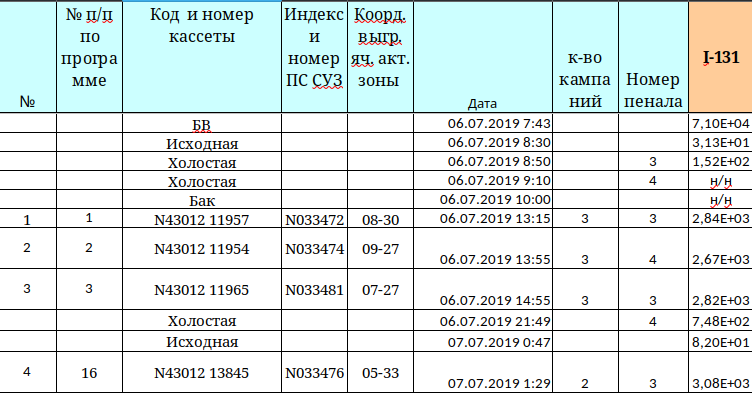
\includegraphics[width=1\linewidth]{pics/ris4} % изображения хранятся в подкаталоге pics
	\caption{Пример входных данных}
	\label{fig:ris4} % эта метка позволяет ссылаться на рисунок в тексте
\end{figure}

\begin{figure}[H]
	\centering
	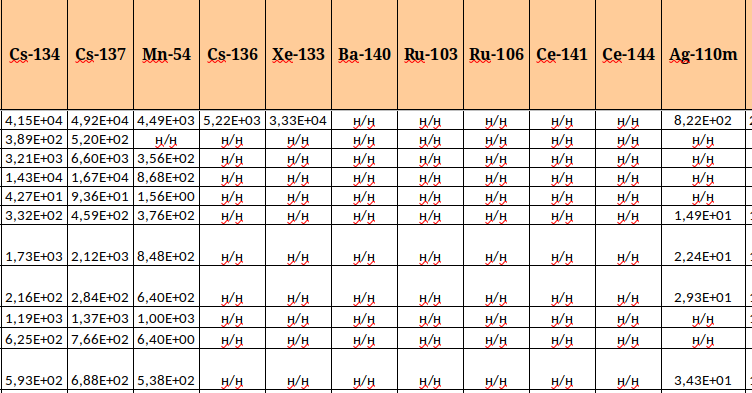
\includegraphics[width=1\linewidth]{pics/ris5} % изображения хранятся в подкаталоге pics
	\caption{Пример входных данных}
	\label{fig:ris5} % эта метка позволяет ссылаться на рисунок в тексте
\end{figure}

Как видно из примера, входные данные содержат строки и столбцы, которые используются в других расчётах. Следовательно, для использования в приложении эти данные необходимо очистить. 

Чтение файла из табличных файлов(таких как .xls, .xlsx, .ods) реализовано в методе read\_excel() библиотеки pandas. Данная функция возвращает объект DataFrame, который передаётся в метод очистки под определённый шаблон входных данных. Фрагмент реализация метода, отвечающего за очистку DataFrame представлена на листинге~\ref{lst:1}. 

\begin{flushleft}
\needspace{3\baselineskip}
\captionof{Program}{Метод очистки данных} \label{lst:1}
\begin{MyCodes}
def _clear_data(self, df):
	# На текущий момент данные очищаются под конкретный шаблон пробных данных.
	# Делаем срез DataFrame, используем первые 14 столбцов
	df = df.iloc[:,0:14] 
	# Переименовываем столбцы для удобного анализа
	df.rename(columns = {
		"№":"Id1",
		"№ п/п по программе":"Id2",
		"Код  и номер кассеты":"Name",
		"Индекс и номер ПС СУЗ":"Index",
		"Коорд. выгр. яч. акт. зоны ":"Coordinates",
		"Дата":"DateTime",
		"к-во кампаний":"Age",
		"Номер пенала":"IdPenal"}, inplace = True)
	
	for i in range(0, len(df.columns.to_list())):
		column = df.columns.to_list()[i]
		df.replace({column:"-"}, np.NaN, inplace=True) # Заменяем спец. символы
		df.replace({column:"н/н"}, np.NaN, inplace=True)
	
	# Заполняем пропуски и приводим типы
	df["Age"]=df["Age"].fillna(0.0).astype(int)
	df["IdPenal"]=df["IdPenal"].fillna(0.0).astype(int)
	df["Id2"]=df["Id2"].fillna(0.0).astype(int)
	
	...
	
	return penals, penals_id, cassetes

\end{MyCodes}
\end{flushleft}

\subsection{Анализ данных}

\subsubsection{Поиск выбросов}

Поиск выбросов в разрабатываемом приложении реализован в качестве метода у сущности, представляющей выборку. Метод основан на вычислении критического значения для выборки по заданному критерию. После вычисления критического значения объект DataFrame агрегируется по условию. Полученные строки удаляются из исходного DataFramе и производится повторный расчёт критического значения согласно параграфу~\ref{povtor}. 

Фрагмент реализации метода поиска выбросов, связанный с расчётом критических значений представлен в листинге~\ref{lst:check}.

\begin{flushleft}
	\needspace{3\baselineskip}
	\captionof{Program}{Фрагмент метода поиска выбросов} \label{lst:check}
	\begin{MyCodes}
...

# method_type - аргумент функции, указывающих метод поиска выбросов
if method_type=="IQR":
Расчёт параметров для метода "IQR"
	a_q1 = df[criteriums[i]].quantile(q=.25)
	a_q3 = df[criteriums[i]].quantile(q=.75)
	a_IQR = a_q3-a_q1
	
	a_corosion_q1 = df[criteriums[i]].quantile(q=.25)
	a_corosion_q3 = df[criteriums[i]].quantile(q=.75)
	a_corosion_IQR = a_corosion_q3-a_corosion_q1
	
	a_crit = (a_q3+1.7*a_IQR)
	a_corosion_crit = (a_corosion_q3+1.7*a_corosion_IQR)
else:
	#Расчёт параметров для метода "3 сигм"
	a_mean = df[criteriums[i]].mean()
	a_corosion_mean = df["Mn-54"].mean()
	a_std = df[criteriums[i]].std()
	a_corosion_std = df["Mn-54"].std()
	a_crit = self.crit_value(a_mean, a_std, len(df))
	a_corosion_crit = self.crit_value(a_corosion_mean, a_corosion_std, len(df))

crit_df = df[(df[criteriums[i]]>a_crit)].reset_index(drop=True)
non_hermetic = crit_df[crit_df["Mn-54"]<a_corosion_crit]
recheck = crit_df[crit_df["Mn-54"]>=a_corosion_crit]

...
	\end{MyCodes}
\end{flushleft}

Результатом выполнения данного метода являются 3 таблицы DataFrame:
\begin{itemize}
	\item Таблица негерметичных ТВС, содержит исходные данные о ТВС, а так же радионуклиды, на основании которых предполагается негерметичность.
	\item Таблицы ТВС для повторной проверки, содержит исходные данные о ТВС, а так же радионуклиды, на основании которых предполагается негерметичность.
	\item Таблица расчётных параметров, содержащая информацию о математическом ожидании, среднеквадратическом отклонении, а так же о квантилях.
\end{itemize}

\subsubsection{Статистические тесты}

Все статистические тесты, описанные в 2.2.2-2.2.4, реализованы в библиотеке scipy.stats, что довольно сильно упрощает реализацию данного модуля. Основной задачей во время разработки данного модуля являлось определение достаточного количества повторений тестов(Манна-Уитни и Крамера-Уэлча) согласно алгоритму, предложенному в 2.2.3. Увеличение количества повторений существенно замедляет работу модуля, но в то же время малое число повторений не обеспечивает требуемой точности. 

На основе модельных данных, я проводил тесты для 3 выборок и сравнивал длины доверительных интервалов для N от 10 до 1000 повторений. По результатам исследования было установлено, что:
\begin{itemize}
 \item при изменении числа повторений с 10 до 100, длина доверительного интервала при уровне значимости $\alpha = 0,05$ длина доверительного интервала изменяется в среднем на $\approx 0,2-0,3$ и составляет $\approx 0,05$. Время выполнения метода при этом в среднем изменяется на 0,4 секунды
 
 \item при изменении числа повторений от 100 до 1000, длина доверительного интервала при уровне значимости $\alpha = 0,05$ длина доверительного интервала изменяется в среднем на $\approx 0,02-0,03$ и составляет $\approx 0,018$. Время выполнения метода при этом в среднем изменяется на 2,1-2,5 секунды.
 
\end{itemize}

В результате данного испытания я пришёл к выводу, что длина доверительного интервала $\approx 0,05$ является приемлемой, поэтому выбрал количество повторений N=100. Реализация теста по критерию Манна-Уитни представлена в листинге \ref{lst:mann-whitney}.

\begin{flushleft}
	\needspace{3\baselineskip}
	\captionof{Program}{Реализация теста Манна-Уитни} \label{lst:mann-whitney}
	\begin{MyCodes}
def mannwhitney_test(self, criterium):
	pvalues = []
	
	for i in range(0,100):
		n1, n2 = random_generate(self.df, criterium)
		
		statistic, pvalue = stats.mannwhitneyu(n1, n2, alternative='two-sided')
		
		pvalues.append(pvalue)
	
	pvalues = pd.Series(pvalues)
	pvalue = pd.Series(pvalues).mean()
	confidence = stats.norm.interval(confidence=0.95, loc=np.mean(pvalues),
		scale=stats.sem(pvalues))
	
	return (format(confidence[0], '.3f'), format(confidence[1], '.3f'))
	
	\end{MyCodes}
\end{flushleft}


\subsection{Пользовательский интерфейс}

Данный раздел содержит описание инструментов и трудностей, с которыми я столкнулся во время разработки приложения, а также примеры реализаций графических элементов, используемых в моём приложении.

\subsubsection{Основные окна приложения}

На основании анализа пользовательского сценария использования, представленного в \ref{Scenarii}, был сделан вывод, что проектируемое приложение будет состоять 4 окон(2 основных и 2 диалоговых):

\begin{itemize}
	\item Диалоговое окно импорта файла
	\item Окно анализа пеналов
	\item Окно анализа выборок
	\item Диалоговое окно с результатами статистических тестов 
\end{itemize}

Хочу отметить, что разделение окна анализа выборок и окна анализа пеналов сделано намеренно, т.к. при переходе в окно анализа выборок должна сохраняться не только возможность выбрать выборки заново без изменения в логике. Кроме того подразумевается, что работа по пеналам может проводиться параллельно, следовательно, именно поэтому окно анализа выборок было решено сделать самостоятельным окном, а не интегрировать внутрь другого.

\subsubsection{Окно импорта файла}

При открытии файла используется класс QFileDialog, который предоставляет окно выбора файла. Удобство этого класса заключается в том, что имеется возможность установить фильтры на расширения файлов, чтобы не вызывать исключений при попытке открыть файл с расширением, которое не поддерживается. Пример окна для выбора фала представлен на рисунке~\ref{fig:ris7}.

\begin{figure}[H]
	\centering
	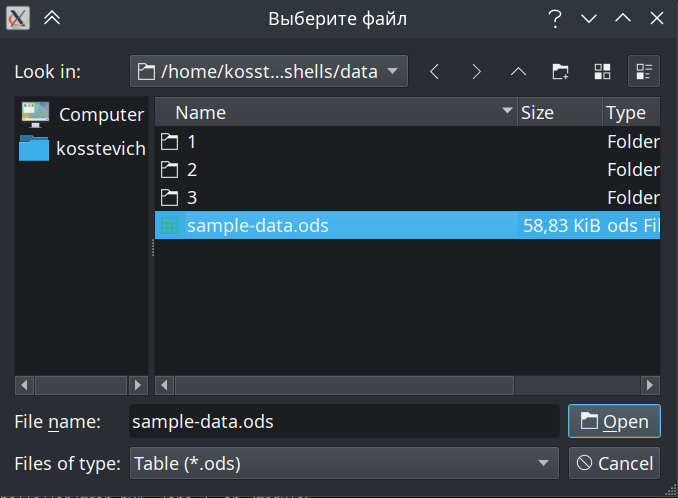
\includegraphics[width=1\linewidth]{pics/ris7} % изображения хранятся в подкаталоге pics
	\caption{Окно выбора файла}
	\label{fig:ris7} % эта метка позволяет ссылаться на рисунок в тексте
\end{figure}

\subsubsection{Интеграция Matplotlib в качестве QWidget}

Во время разработки приложения я столкнулся с трудностью интеграции графиков Matplotlib в QWidjet. Проблема заключалась в том, что базовый класс Matplotlib создаёт для графиков независимые окна. Данная реализация мне не подходит, т.к. разрабатываемое приложение должно иметь целостный формат.

Изучив документацию библиотеки, я нашёл класс FigureCanvasQTAgg, предоставляющий backend-реализацию холста Canvas для PyQt. На основе него был разработан собственный пользовательский виджет для использования в моём приложении. Реализация пользовательского виджета представлена в листинге~\ref{lst:canvas}

\begin{flushleft}
\needspace{3\baselineskip}
\captionof{Program}{Пользовательский класс, интегрирующий Сanvas в QWidget} \label{lst:canvas}
\begin{MyCodes}
class PlotData(FigureCanvasQTAgg): 
	# Виджет для отрисовки графиков, использующий matplotlib
	def __init__(self, parent=None):
		sns.set(style="whitegrid", context="paper")
		self.fig = plt.figure(figsize=(15, 10))
		self.axes = self.fig.add_subplot(111)
		super(PlotData, self).__init__(self.fig)
	
	def draw_plot(self, df, axe_x="Id1",
			axe_y="I-131", type = "barplot", name=None):
		self.axes.cla()
		# Метод позволяет рисовать разные виды графиков seaborn
		# Выбор типа графика происходит по аргументу type
		getattr(sns,type)(data=df, x=axe_x, y=axe_y, ax=self.axes)
		plt.title(label= name, fontsize=16)
\end{MyCodes}
\end{flushleft}

Кроме реализации холста я использовал класс NavigationToolbar2QT, который предоставляет возможности навигации, редактирования легенды, а также экспорт графика в формате изображения. На рисунке~\ref{fig:ris8} красной рамкой выделены реализованные мною классы.

\begin{figure}[H]
	\centering
	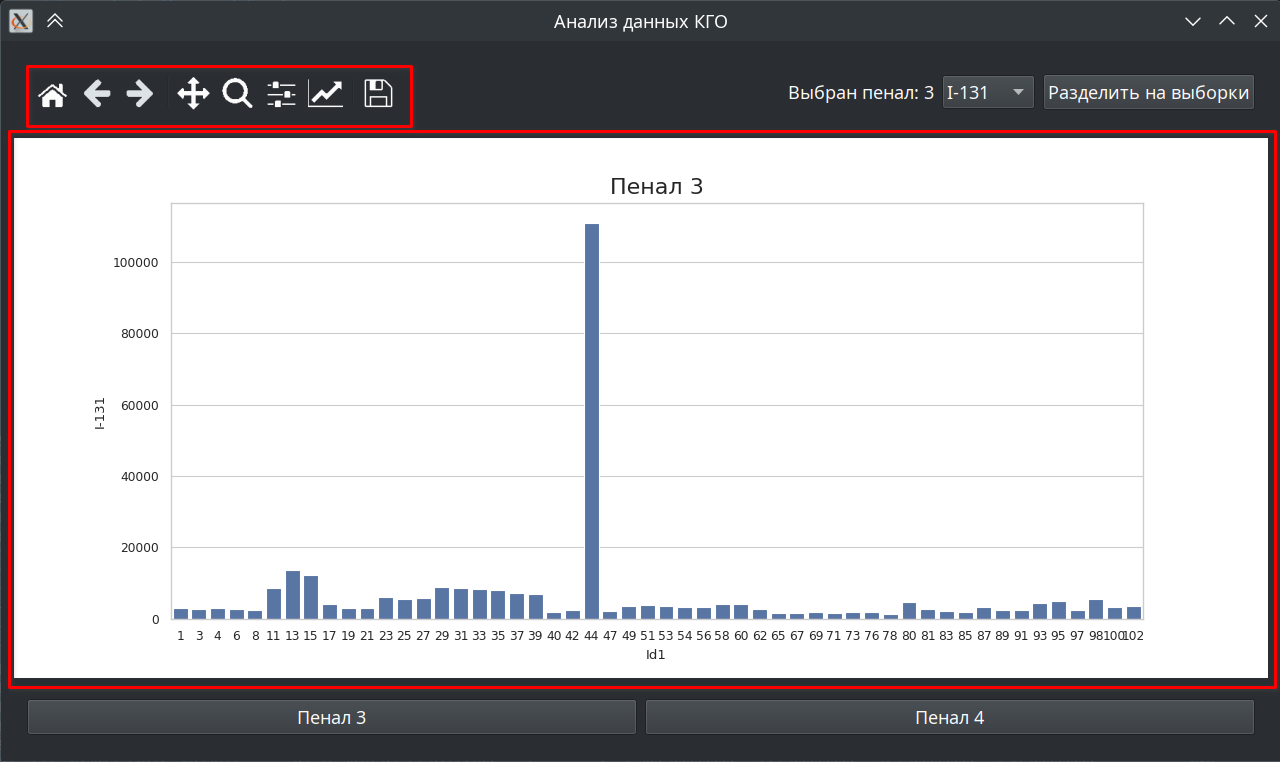
\includegraphics[width=1\linewidth]{pics/ris8} % изображения хранятся в подкаталоге pics
	\caption{Главное окно приложения}
	\label{fig:ris8} % эта метка позволяет ссылаться на рисунок в тексте
\end{figure}

\subsubsection{Главное окно приложения}

Пример внешнего вида главного окна приложения приведён на рисунке \ref{fig:ris8}. Данное окно реализовано с использованием элементов Qt:

\begin{itemize}
	\item QPushButton --- класс, отвечающий за кнопку.
	\item QLabel --- класс, позволяющий выводить текстовую информацию.
	\item QComboBox --- класс, реализующий выпадающий список.
	\item QHBoxLayout --- класс, позволяющий располагать виджеты в горизонтальной разметке
	\item QVBoxLayout --- класс, позволяющий располагать виджеты в вертикальной разметке
\end{itemize}

Кнопки, отвечающие за переход по пеналам, реализованы динамически в зависимости от количества пеналов в исходных данных.

\subsubsection{Окно анализа выборок}

Пример реализации окна анализа выборок представлен на рисунке~\ref{fig:ris10}.

\begin{figure}[H]
	\centering
	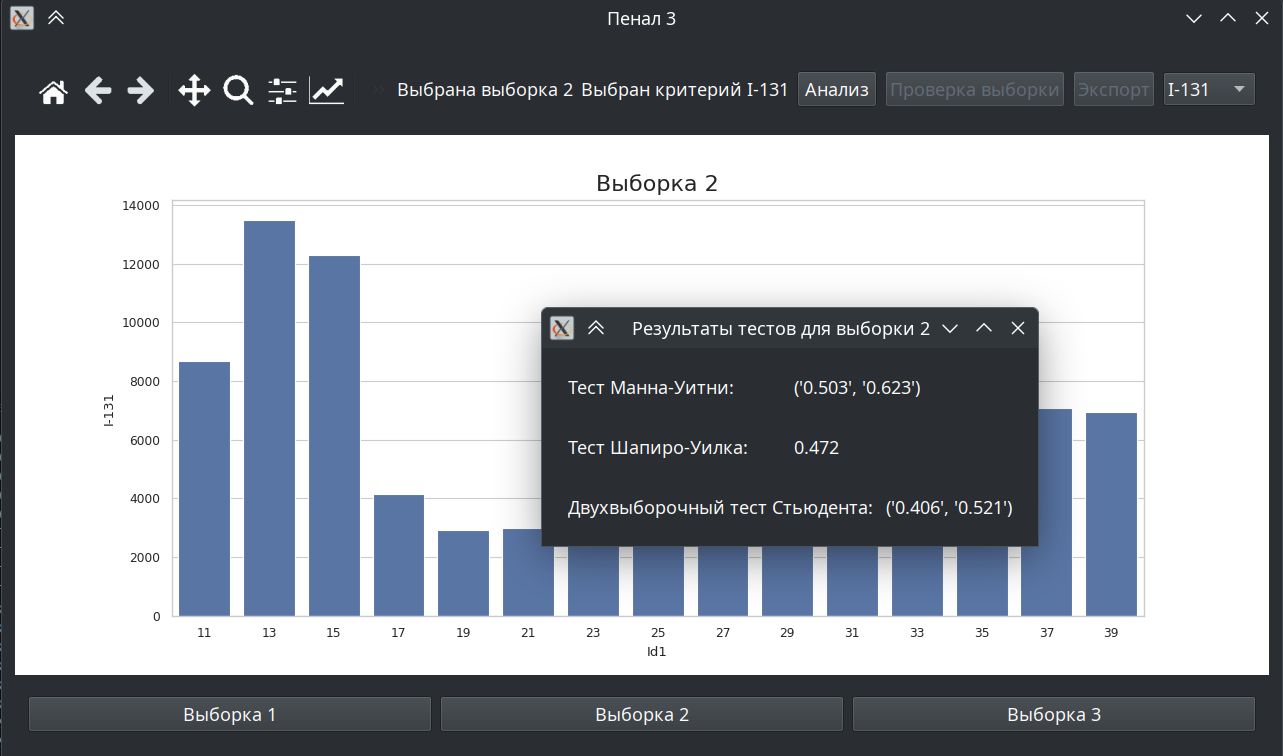
\includegraphics[width=1\linewidth]{pics/ris10} % изображения хранятся в подкаталоге pics
	\caption{Окно анализа выборок}
	\label{fig:ris10} % эта метка позволяет ссылаться на рисунок в тексте
\end{figure}

Несмотря на схожесть с окном анализа выборок, данное окно имеет более сложную структуру. В частности, класс PlotData, описанный в 4.4.3, после проведения поиска выбросов заменяется на класс QTableWidget, который содержит выходную информацию в табличном виде. Данный функционал реализован с применением класса QStackedWidget, который позволяет отображать только один из нескольких дочерних объектов. Пример табличного вывода представлен на рисунке~\ref{fig:ris14}.

\begin{figure}[H]
	\centering
	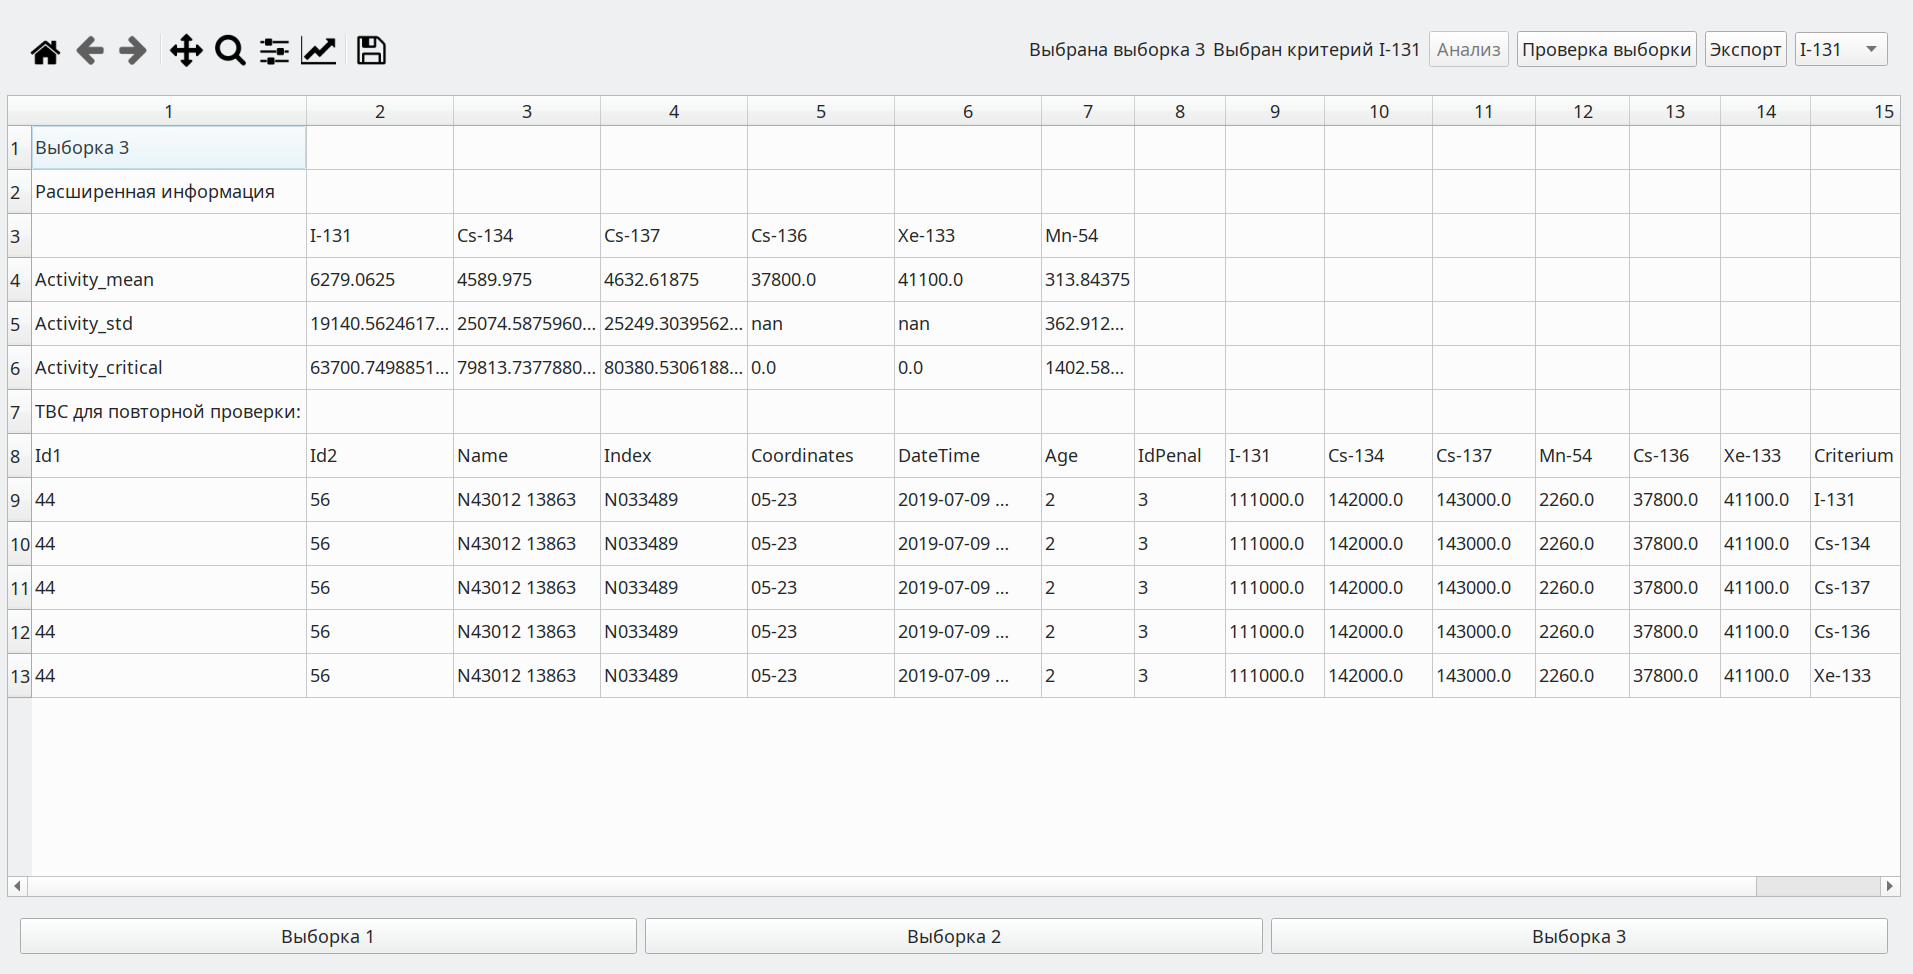
\includegraphics[width=1\linewidth]{pics/ris14} % изображения хранятся в подкаталоге pics
	\caption{Представление табличной информации через QTableWidget}
	\label{fig:ris14} % эта метка позволяет ссылаться на рисунок в тексте
\end{figure}

После проведения необходимого анализа, имеется возможность экспорта таблицы в .ods формат. Пример экспортированного файла приведён на рисунке~\ref{fig:ris12}.

\begin{figure}[H]
	\centering
	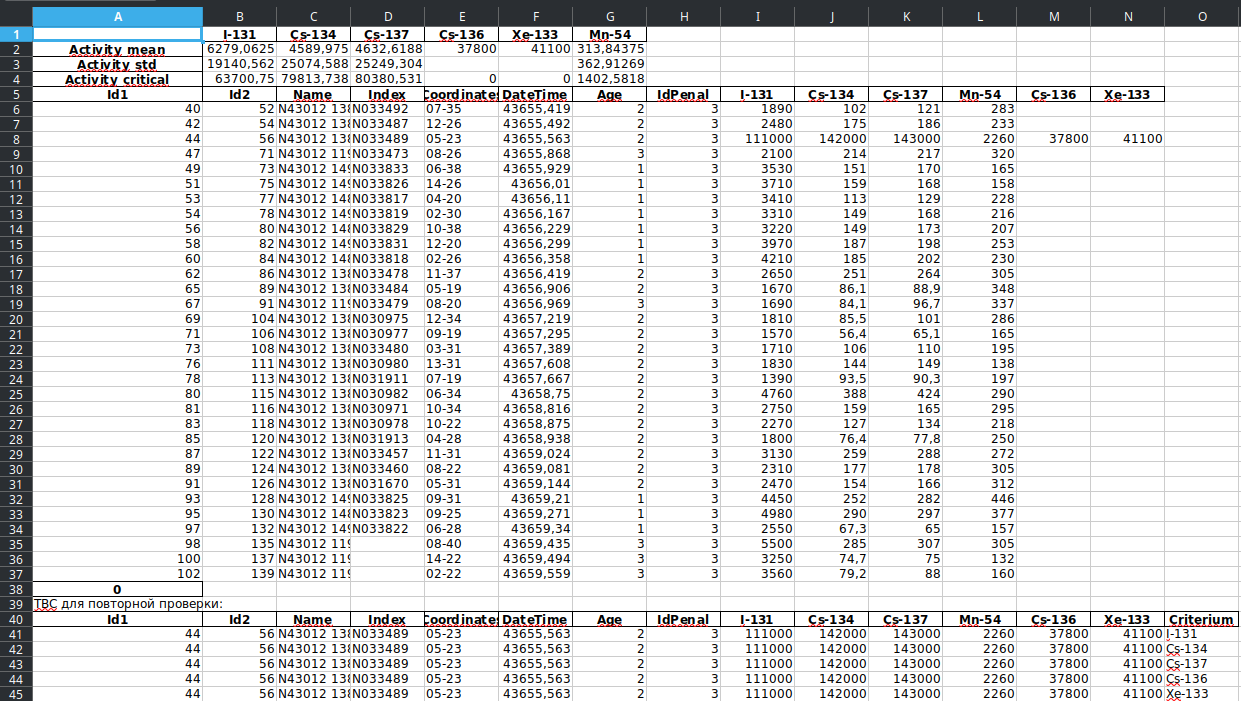
\includegraphics[width=1\linewidth]{pics/ris12} % изображения хранятся в подкаталоге pics
	\caption{Пример выходного файла}
	\label{fig:ris12} % эта метка позволяет ссылаться на рисунок в тексте
\end{figure}

%Интеграция графиков Matplotlib в QtWidget % четвертая глава - в файле part4.tex
%\pagebreak

%\input{part5}  % пятая глава - в файле part5.tex
%\pagebreak

\section*{\centering ЗАКЛЮЧЕНИЕ}
\addcontentsline{toc}{section}{ЗАКЛЮЧЕНИЕ}

В ходе проделанной работы была проведена --- описать результаты бурной деятельности по выполнению ВКР, разумно в виде списка выполненных задач.

Разработанная программа позволяет --- перечислить основные функциональные характеристики и особенности, можно в виде списка:
\begin{itemize}
\item выполнено такое-то задание;
\item разработана некоторая система;
\item у работы есть перспективы развития.
\end{itemize}

% оформление библиографии - вариант с БД
\pagebreak

\addcontentsline{toc}{section}{СПИСОК ИСПОЛЬЗОВАННЫХ ИСТОЧНИКОВ}
% ВАЖНО: для корректного отображения в списке литературы ссылок на англ.языке в bibtex-описание источника следует добавить поле 
% langid = {english}
\printbibliography

\pagebreak

\renewcommand{\appendixpagename}{\centering Приложения}

\begin{appendices}
\renewcommand{\thesection}{\Asbuk{section}}
\makeatletter
\renewcommand{\theProgram}{\thesection.\@arabic\c@Program}
\makeatother

% каждое приложение задается следующей командой, нумерация - русскими буквами
\section{\centering } 
% независимая нумерация листингов в каждом приложении
\setcounter{Program}{0}

\begin{flushleft}
\needspace{3\baselineskip}
\captionof{Program}{ Часть кода реализации класса HashMapValue}\label{app1}
\begin{MyCodes}
public class HashMapValue {
	
	protected String filename; 
	protected HashMap<String, String> hashValue = 
	new HashMap<>();
	protected HashMap<String, Boolean> hashKeysFlag =
	 new HashMap<>();
	
	public void setData(String key, String value) {
		hashValue.put(key, value);
	}
	
	public String getData(String key) {
		return hashValue.get(key);
	}
    /* ... */
}
\end{MyCodes}
\end{flushleft}

\pagebreak

\begin{flushleft}
\captionof{Program}{Пример кода}\label{app2}
\begin{MyCodes}
код второго приложения
\end{MyCodes}

\end{flushleft}
% следующее приложение - раскомментировать команды
%\section{\centering } 
%\setcounter{Program}{0}
%\begin{MyCode}
%код третьего приложения
%\end{MyCode}
%\nopagebreak
%\begin{Program}
%\caption{Еще пример кода}\label{app3}
%\end{Program}

\end{appendices}

\end{document}          

